\section{Exploratory data analysis} \label{sec:explore}
% \hl{Dj: [Generic explanation of the structure of data, i.e. we received data split already; how many data points, how many species. Did each species have equal data points?(No), should address these q's.]}

% \hl{Dj: I think that we will need to be quite particular about what we place in exploratory data analysis -> should be relevant to our tasks.}

% \hl{Dj: whats written below is very rough and will need to be reworded etc..}
A brief overview of the available data structure is included in appendix \ref{appendix:datastruct}. Notably, the mean number of locations attributed to each species is much higher in the test data-set vs. the train data-set. The training data, sourced from citizen scientists, is noisy due to non-regularized collection methods, and important information relevant to  conservation efforts such as the observation date of the species is not provided. 
Additionally, the format of the two data-sets is different. The train data-set provides locations and a singular associated species, whereas the test data-set provides locations and a corresponding list of multiple species. It is important to note the difficulty that this may present in creating models that can accurately predict multiple species per location\footnote{This is because the training data-set provides us with data suited to a singular label classification problem, whereas the test data-set is suited toward a multi-label classification problem.}. The distribution of these two data-sets is best visualized through the plots given in Figure \ref{fig:dist_data}.

\begin{figure}[hbt!]
\centering

\begin{subfigure}{.32\linewidth}
\vspace*{-1ex}  
\begin{center}
\textbf{Train data-set}
\end{center}
\vspace*{-1ex}
  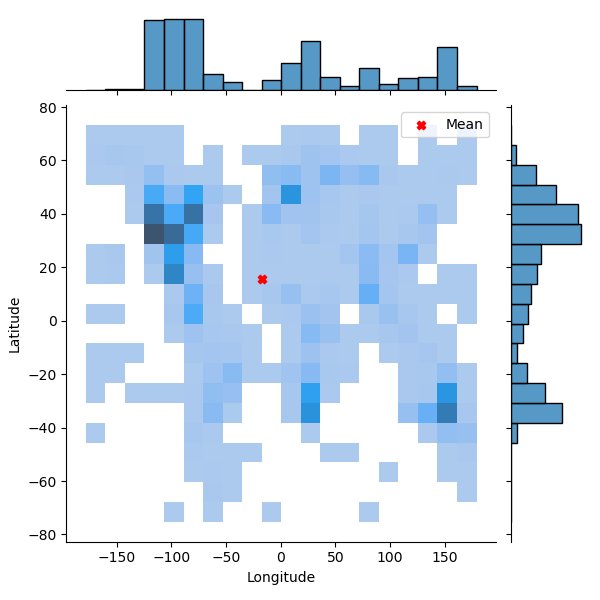
\includegraphics[width=\linewidth]{Images/hist_train.png}
\end{subfigure} % <-- "\hfill"
\begin{subfigure}{.32\linewidth}
\vspace*{-1ex}  
\begin{center}
\textbf{Test data-set}
\end{center}
\vspace*{-1ex}
  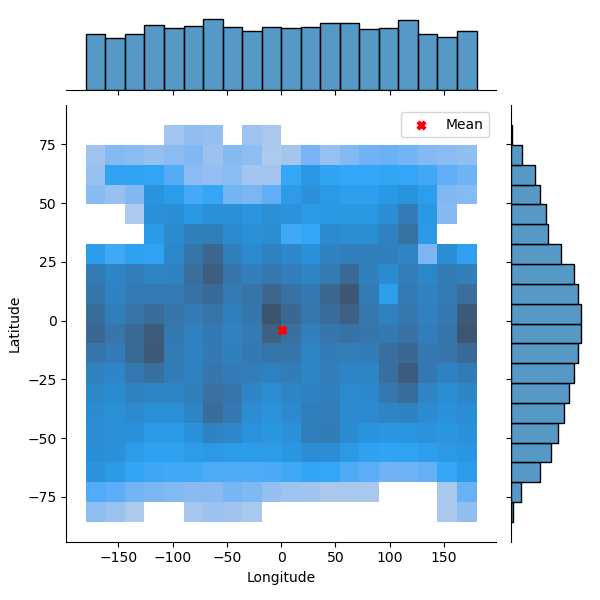
\includegraphics[width=\linewidth]{Images/hist_test.png}
\end{subfigure}
\begin{subfigure}{.32\linewidth}
\vspace*{-1ex}  
\begin{center}
\textbf{Avg. species observations per continent (train data-set)}
\end{center}
\vspace*{-1ex}
  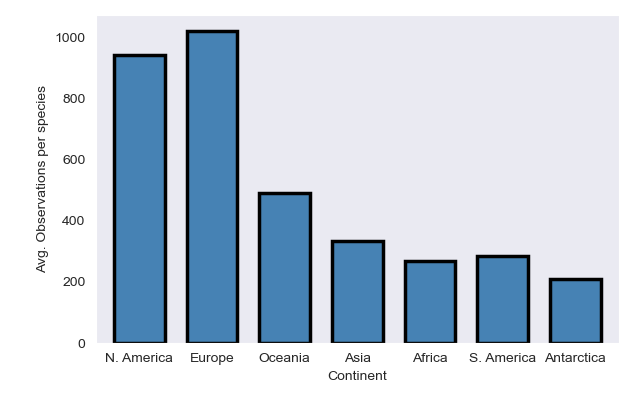
\includegraphics[width=\linewidth]{Images/obsve.png}
\end{subfigure}

\caption{Distribution of data from the train (left) and test (middle) data-sets at locations where there are species observation $\geq$ 1, note the offset mean location in the train data-set, and the centralized mean location in the test data-set. (Right) is a comparison of the number of observations per species in the train data-set for each continent.}
\label{fig:dist_data}
\end{figure}

Data from the training data-set is not evenly spread, with larger amounts of data associated with the longitude and latitude ranges (-120, -90) and (20, 50) for example, roughly corresponding to North America. This can be attributed to the fact that there may be more iNaturalist users in this region.
An analysis on the number of observations per species for each continent is subsequently carried out to further show this data imbalance.
A random sample of twenty locations (converted to a continent name) was taken for every species, and the most common continent among those twenty was taken to be the species continent. As shown in Figure \ref{fig:dist_data}, Europe has the highest number of observations (data-points) per species. This shows a clear bias in the data; species from Europe and North America have, on average, a larger number of observations. A more comprehensive table of this data is included in Appendix \ref{appendix:table1}. The test data-set on the other hand, considers a (roughly) even spread of location data points. Additionally, the species in the data-set have widely varying population distributions. 
Figure \ref{fig:dist} shows the extremes in species distribution span and density in the test data-set.
%Figure \ref{fig:dist} shows an analysis of the population distribution span and density of data in the train data-set, i.e. a comparison of the largest found distances and densities between data points of a species.

\begin{figure}[hbt!]
\centering

\begin{subfigure}{.45\linewidth}
\vspace*{-1ex}  
\begin{center}
\textbf{Species distribution span}
\end{center}
\vspace*{-1ex}
  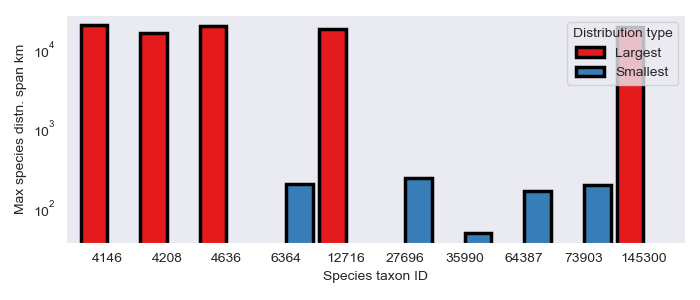
\includegraphics[width=\linewidth]{Images/large_small.png}
\end{subfigure}
\begin{subfigure}{.45\linewidth}
\vspace*{-1ex}  
\begin{center}
\textbf{Species distribution density}
\end{center}
\vspace*{-1ex}
  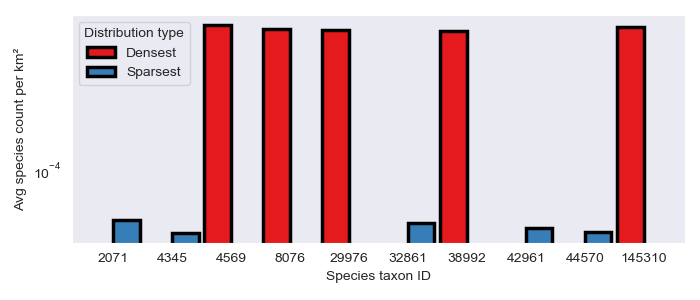
\includegraphics[width=\linewidth]{Images/dense_sparse.png}
\end{subfigure} % <-- "\hfill"

\caption{(Left) The variation on population distribution of 10 different species (top 5 largest vs top 5 smallest). (Right) The variation on population density of 10 different species (top 5 densest vs top 5 sparsest), note the logarithmic scaling of both plots.}
\label{fig:dist}
\end{figure}

Notably, population spans vary widely. An initial hypothesis is that this will affect a machine learning model's ability to correctly predict species distributions\footnote{Largely spread populations may provide less generalization for the ML models to learn about species population.}, and so this is something that we would like to investigate. 
Not only do the species population distributions span different distances, but they also have a wide range of densities. Some species have a much larger count in the train data-set attributed to a smaller area, whereas other species have small counts over larger areas.
A second hypothesis to consider is our machine learning methods' capability to predict sparse and dense population distributions\footnote{Sparsely spread populations provide less correlation for the ML models to learn, whereas dense populations have fewer outliers.}.

%Another way we analysed the data was by looking at the most commonly observed species. There are 64 species in the data-set with \hl{greater than?} 2000 observations (the maximum number). Out of these species, a random sample of 10 locations was taken to compute the most common continent in which these species are located. While 10 points aren’t much, calculating the continent of each coordinate requires a lot of computational power, and each species is “expected” to be mostly in the same continent. We found that most species with max observations were observed in North America with 42 and Europe with 12 while Oceania had 4, Africa and South America 2, and Asia 1. This clearly shows a big bias in where the data was collected. 

%Another way we analysed the data was by searching for the most and least commonly observed species. As shown in \ref{tab:my_continent} there are 72 species with more than 1500 locations. For all species, a random sample of 20 locations was taken to compute the most common continent in which these species were located. North America had the most species overall with 134, Africa was second with 122 and Europe was last with 34 (excepting Antarctica). Yet, for the most common species, Europe comes second to North America with 12 species while Africa only has 2. This shows a very clear bias in the data, while Africa has much more diversity, Europe has many more observations per species.

% \hl{can this paragraph be moved to where I highlighted ----}

% Finally, we analysed the data by searching for the most common continent for each species. A random sample of 20 locations (converted to a continent name) was taken for every species, the most common continent among those 20 was taken to be the species continent. As shown in appendix \ref{appendix:table1}, North America has the most number of species with 134, closely followed by Africa with 122, while Europe has the least with 34 (excepting Antarctica). However, the number of observations in Europe per species nearly quadruples those in Africa. This shows a clear bias in the data; species from Europe and North America have, on average, a lot more observations.% This reinforces the need to balance the data before training our models to prevent the model from being disproportionately influenced by labels from Europe and North America with an abundance of data. %This is consistent with what you would expect from "citizen scientists" as most of the iNaturalist community resides in these continents. 

%\hl{Would be interesting to check later on if we get a better accuracy for North America and Europe compared to the other continents? Is this possible computationally? Would possibly have to check the continent of every location – not realistic computationally. In any case this shows the importance of “data balancing” in some way. We will probably need to create weights for each specie.}


% Don't think we'll need to do the density one
% Additionally, further analysis of the distribution of species was done to analyze the density of populations

% \begin{figure}[h]
% \centering
% \includegraphics[width = \textwidth]{Images/Dense_spread.png}
% \caption{Largest found density of species (Hyla Chinensis) versus smallest (Larus occidentalis).}
% \end{figure}